\documentclass{sigchi}

% Use this command to override the default ACM copyright statement (e.g. for preprints). 
% Consult the conference website for the camera-ready copyright statement.


%% EXAMPLE BEGIN -- HOW TO OVERRIDE THE DEFAULT COPYRIGHT STRIP -- (July 22, 2013 - Paul Baumann)
% \toappear{Permission to make digital or hard copies of all or part of this work for personal or classroom use is 	granted without fee provided that copies are not made or distributed for profit or commercial advantage and that copies bear this notice and the full citation on the first page. Copyrights for components of this work owned by others than ACM must be honored. Abstracting with credit is permitted. To copy otherwise, or republish, to post on servers or to redistribute to lists, requires prior specific permission and/or a fee. Request permissions from permissions@acm.org. \\
% {\emph{CHI'14}}, April 26--May 1, 2014, Toronto, Canada. \\
% Copyright \copyright~2014 ACM ISBN/14/04...\$15.00. \\
% DOI string from ACM form confirmation}
%% EXAMPLE END -- HOW TO OVERRIDE THE DEFAULT COPYRIGHT STRIP -- (July 22, 2013 - Paul Baumann)


% Arabic page numbers for submission. 
% Remove this line to eliminate page numbers for the camera ready copy
% \pagenumbering{arabic}


% Load basic packages
\usepackage{balance}  % to better equalize the last page
\usepackage{graphics} % for EPS, load graphicx instead
\usepackage{times}    % comment if you want LaTeX's default font
\usepackage{url}      % llt: nicely formatted URLs

% llt: Define a global style for URLs, rather that the default one
\makeatletter
\def\url@leostyle{%
  \@ifundefined{selectfont}{\def\UrlFont{\sf}}{\def\UrlFont{\small\bf\ttfamily}}}
\makeatother
\urlstyle{leo}


% To make various LaTeX processors do the right thing with page size.
\def\pprw{8.5in}
\def\pprh{11in}
\special{papersize=\pprw,\pprh}
\setlength{\paperwidth}{\pprw}
\setlength{\paperheight}{\pprh}
\setlength{\pdfpagewidth}{\pprw}
\setlength{\pdfpageheight}{\pprh}

% Make sure hyperref comes last of your loaded packages, 
% to give it a fighting chance of not being over-written, 
% since its job is to redefine many LaTeX commands.
\usepackage[pdftex]{hyperref}
\hypersetup{
pdftitle={MACHINE-ASSISTED COOKING},
pdfauthor={LaTeX},
pdfkeywords={SIGCHI, proceedings, archival format},
bookmarksnumbered,
pdfstartview={FitH},
colorlinks,
citecolor=black,
filecolor=black,
linkcolor=black,
urlcolor=black,
breaklinks=true,
}

% create a shortcut to typeset table headings
\newcommand\tabhead[1]{\small\textbf{#1}}


% End of preamble. Here it comes the document.
\begin{document}

\title{Machine-Assisted Cooking}


%\numberofauthors{1}
%\author{
%  \alignauthor Miriam Cha, Michelle Deng, and Melih Elibol\\
%    \affaddr{Harvard University}\\
%    \affaddr{Cambridge, MA 02138}\\
%    \email{\{miriamcha, michelledeng, melihelibol\}@g.harvard.edu}\\
%}

\numberofauthors{3}
\author{
  \alignauthor Miriam Cha\\
    \affaddr{Harvard University}\\
    \affaddr{Cambridge, MA 02138}\\
    \email{miriamcha@fas.harvard.edu}\\
  \alignauthor Michelle Deng\\
    \affaddr{Harvard College}\\
    \affaddr{Cambridge, MA 02138}\\
    \email{mdeng@college.harvard.edu}\\
  \alignauthor Melih Elibol\\
    \affaddr{Harvard Extension School}\\
    \affaddr{Cambridge, MA 02138}\\
    \email{elibol@fas.harvard.edu}\\
}

\maketitle

\begin{abstract}
We present the observations, processes, and results in designing a machine assisted cooking interface for novice chefs. We present detailed observations from our user experiments and the resulting evolution in our interface design. We describe the final interface that is the result of this process, and list important features that contributed to its success. We conclude with the current state of our work and our plans for the future. 
\end{abstract}

%\keywords{
%	sensemaking; instructions; author's kit; conference publications;
%	keywords should be separated by a semi-colon. \newline
%}
%
%\category{H.5.m.}{Information Interfaces and Presentation}{Miscellaneous}

%See: \url{http://www.acm.org/about/class/1998/}
%for more information and the full list of ACM classifiers
%and descriptors. \newline
%\textcolor{red}{Optional section to be included in your final version, 
%but strongly encouraged. On the submission page only the classifiers’ 
%letter-number combination will need to be entered.}

\section{Introduction}

For decades now, food options in America have been primarily unhealthy. Unhealthy food options have grown from fast food restaurants to web-based delivery services. It has become increasingly easy to eat unhealthy food, and this is a problem for people who want to make a change. In this regard, there is a need for healthier eating. There are several ways to address this issue, one of which is to simply make your own food. To enable those who are motivated but inexperienced with cooking, the process of learning to prepare a home cooked meal must first  be well understood. Most people today learn to cook by following a recipe book, or reading recipes online. To better understand the process of learning to cook, as well as understand good cooking practices, we observed three subjects with varying cooking experience cook a meal following a recipe with which they were unfamiliar. Our observations showed that even experienced cooks exhibit symptoms of cognitive overload, which lead to mistakes, frustation, and in one case, a loss in motivation to cook. One major cause of such symptoms is poor recipe instruction. Consequently, the primary focus of this work is to improve the experience of learning a new recipe by improving the design of recipe instruction.

***** NOTE ***** Should the rest of this come after related work / be incorporated into related work?

Our examination of popular recipes showed such recipes are typically geared toward people who have sufficient experience cooking. The typical recipe lists out ingredients needed and either gives a paragraph describing what needs to be done, or a coarse list of steps that need to be carried out. Based on cognitive-load-theoretic principles, and work done by Mayer \cite{mayer_2003}, cognitive load due to cooking and following instruction simultaneously may be reduced by reducing the amount of information displayed at any given time, called chunking. The use of interactive media is a natural way to chunk information.

Work on adaptive graphical user interface techniques \cite{gajos_2005, gajos_2006, tsandilas_2005} show that highlighting what the user is predicted to be looking for decreases search time. We make use of adaptive techniques by emphasizing the current step being carried out in the cooking process. We also emphasize the ingredients needed for that step. % To further improve search-time, interface states resulting from recipe interactions were animated, which allowed for ...

Our observations show that cooking is very much a process over which multiple tasks are executed simultaneously. The need for a performant user interface is therefore important. We measure the interactive performance of our interfaces using Fitts' law \cite{fitts_1954}, which can be described as the time $MT$ it takes to acquire a target of a particular size $A$ and distance $W$ according to the following equation $MT = a + b log_2{\frac{A}{W}+1}$. In general, improvements were made to target hit areas (increase hit area greater than actual UI elements), variability in target positioning (spatial consistency of menu item positions), and minimizing the overall amplitude required to navigate between steps by introducing alternatives to point-and-click navigation (natural scrolling).

The major experimental feature of our interface is the use of Semantic Zoom (SZ) ************************\cite{semantic_zoom}: A technique for mangifying (or demagnifying, in our case) not only the geometric properties of data, but also the structure and selection of data. We believe our use of semantic zoom is a form of interface adaptation which emphasizes relevant information while maintaining accessibility to logically adjacent information. We present our findings on the effectiveness of our SZ interface over a more traditional / stable version of an interface that chunks instructions.

[Possibly need some details on reason and value of subgoaling. Make sure to cite the paper Gajos sent out.]

There were aspects of recipe instruction that were left unchanged. We retained what was good and improved what was missing.

%***** NOTE ***** Not sure we need this information 
%Paragraph-based layouts possess little structure with respect to instruction. A more common layout is to list instructions in steps, and display a separate list of ingredients. These new layouts exploit the inherent structure in cooking, which seems natural. This is also a very common layout pattern with which people have grown accustomed to. Retaining some familiarity to this layout is important for reasons that go beyond the scope of this paper.

%****** START ****** Notes on cognitive load
%Based on cognitive-load-theoretic principles, we believed this would make the cooking process easier. We also believed that allowing the user to maintain some global sense of progress was also important.

%The observational results of our studies led us to model the process of cooking as follows. The three main components of cooking are materials, ingredients, and instruction steps. There are X ways to decrease extraneous cognitive load and increase germane cognitive load.

%Much of the process involved in cooking is inherently step-by-step (procedural/sequential). In general, for each step, a process is carried out using a set of materials and ingredients. Some processes carried out by each step may be parallelized: Such steps that they do not depend on each other (they have no topological relation). We view these as advanced techniques that complicate the cooking process. In turn, we believe an examination of parallelization goes beyond the scope of this paper and contributes little to effective improvements in the instructional design of recipes for people who lack sufficient cooking experience.

%Given the aforementioned model, it's clear that a set of materials and ingredients are needed for each step, and each step is ordered temporally. There is also a relation between the set of materials and ingredients used in each step. These relations illustrate a schema for the process of cooking. Based on this schema, we can improve the instruction of recipes by focusing on the development of the aforementioned relationships, and in turn, enable new cooks to learn the same structures associated with cooking that enable experts to rapidly organize and execute recipes they've never cooked before.
%****** END ****** Notes on cognitive load

%****** START ****** Old Intro
%Cooking can be a source of enjoyment as well as a forum for creative experimentation. Compared to prepackaged and most restaurant meals, homemade meals are undoubtedly healthier, economical, and give more control over what goes into one's plate. Unfortunately, home cooking has been increasingly perceived to be too stressful and time-consuming, therefore not worthy of the trouble. Developing the proper skills to cook with confidence takes time and patience. The tools, ingredients, motor skills, effective use of heating/cooling appliances, pressures of precise timing, importance of precise timing, as well as several other factors may seem overwhelming to novices. 

%The vast majority of novice chefs learn to cook using printed cookbooks and websites. Recipes in printed cookbooks are often presented in a paragraph or a list format. There are many cooking blogs or websites \cite{allrecipes, cooking_classy} that share recipes. Online recipes tends to be merely a digital version of printed cookbooks, presenting recipes in paragraphs or lists. We believe the traditional curation of a recipe increases cognitive load while cooking. With the traditional recipe design, one needs to foresee previous, current, and future ingredients and instructions in order to cook without constant interruption. Some novice chefs use cellphone applications [cite1, cite2]. For example, Cook Assistant Lite \cite{cook_lite} makes cooking interactive by only presenting current instructions and ingredients, which is different from the traditional curation of a recipe. However, only presenting an active step requires the user to continually interact with the application, which leads to frequent interruptions while cooking. 

%For this work, we design a user interface for a machine assisted cooking application. The interface is improved upon series of detailed observations of novice chefs cooking. The goal of our interface is reducing unnecessary cognitive load thorough effective recipe presentation. Our design focuses on the curation of instructions and ingredients. 

%Prior to our work, little research has been devoted to understand the ideal curation of a recipe. 

%Getting your first meal right is challenging without help, and failure may discourage people from trying again. There are few resources that currently exist which help mitigate the cognitive load experienced by first-time cooks. For instance, printed cookbooks increase cognitive load, because ingredients and instructions must be memorized in order to cook without interruption. Cooking blogs (e.g., \cite{cooking_classy, allrecipes}) provide plenty of recipes and guides, but these sources are merely digital versions of printed cookbooks. Cook Assistant Lite is one cellphone application that has made cooking interactive \cite{cook_lite}, but the application requires the user to continually interact with the application, which leads to even more interruptions while cooking.
%
%In this paper, we propose a digital cooking assistant design for novice cooks. Our design focuses on the following points:
%\begin{itemize}
%\item	Mitigate interruptions that are due to overutilization of visual input (necessary visual observations while cooking and having to continually read something to determine what to do next) and motor functions (hands are used for cooking and clicking through applications or scrolling on a blog).
%\item Mitigate cognitive overload that is due to the physical and temporal demands of cooking, which are exacerbated by the memorization of ingredients and instructions.
%\item Make instructions in recipes more accessible, teach users new cooking techniques, and help users decide what to make with the ingredients they already have at home.
%\end{itemize}
%
%Features of our design include text-to-speech instruction; timers for managing multiple simultaneous tasks; reminders to check oven and stove temperatures; easy-to-read interfaces that display one step at a time with large pictorial, audio, and/or video aids, somewhat reminiscent of turn-by-turn navigation of a GPS; and lifelines to contact other users who have previously tried the recipe.
%
%Our approach is user-centered. We survey both novice and expert cooks in order to identify key differences between skill levels. For instance: What do novice cooks find most difficult about cooking? What prevents them from cooking more often? What motivates experts to cook? Survey results inform our design of several paper-based interfaces. We then conduct a round of in-person questionnaires to obtain feedback on multiple paper-based designs, which help to identify prominent features and issues with each design. We show multiple designs in parallel to each participant. After incorporating feedback on paper prototypes, we implement the digital design leveraging the recipe API BigOven \cite{api_oven}. To assess the quality of our digital prototype(s), we conduct a within-subject experiment, comparing user performance on cooking recipes with and without our prototype(s). During the performance phase, we collect qualitative data by observation. After each cooking session, we ask the user to assess their cooking experience based on the following factors (NASA Task Load Index): mental demand, physical demand, temporal demand, performance, effort, and frustration. Finally, through further user testing and design/development iteration, our final product embodies the features that help first-time and novice cooks succeed in their cooking adventures.
%****** END ****** Old Intro

\section{Related Work}

Cognitive theory has been extensively studied in the field of instructional interface design. The majority of work is based on Baddeley'��s canonical model of working memory as a limited buffer for visual and auditory information \cite{baddeley_1992}. When the buffer is overloaded, possibly by performing tasks that involve an ordered series of physical and mental activities, new information can fail to be processed \cite{baddeley_1992, miller_1956}. Mayer expands Baddeley'��s model to form a cognitive theory of multimedia learning \cite{mayer_2003}. In his model, information processing is divided into a verbal (not necessarily auditory) channel and a visual channel. Again, each channel has a fixed information-processing capacity and can be overloaded. Mayer presents a series of principles for designing instructional multimedia aimed to reduce cognitive effort required from the learner for one or more channels \cite{mayer_2005}.

Over the last decade, similar principles have often been used in the design of multimedia systems for academic or conceptual instruction (e.g., Moons et al. \cite{moons_2013} or Wong et al. \cite{wong_2012}). However, unlike academics, most activities, cooking included, require less intellectual effort but require coordination of motion and sensation. The requirements on the channels of information processing thus differ. Paas and Sweller \cite{pass_2012} argue that ``biologically primary'' skills passed through evolution require less cognitive effort than explicitly learned, often culturally driven ``secondary'' skills. Based on time of historical emergence, movement-based activities like sports and cooking should be more primary than many fields of academics. On the other hand, Post et al. \cite{post_2013} find that gesturing while watching grammar-instruction animations interferes with learning, and grammar could arguably be a primary skill. Moreover, interference from over loading could be bidirectional, for it is well established that secondary in-vehicle activities such as phoning or texting compromises driver's ability to react to road conditions, leading to injuries and fatalities \cite{brunken_2003}.

Several questions arise, yet few studies have directly investigated the cognitive load effects of teaching tools in non-academic situations. In a rare study, Khacharem et al. \cite{khacharem_2014} investigate the cognitive load effects of animations used for soccer instruction and find that novice players process both static images better than animations and slow animations better than fast ones, whereas expert players learn more effectively with fast animations. Their results suggest that speed and motion from instruction alone can add additional tolls on cognitive load, but these instructions were conveyed offline, as opposed to during gameplay.

The body of literature on cooking instruction is similarly patchy. Recipe recommendation and generation are well documented in the literature \cite{freyne_2010, van_2011, ueda_2011}; many such systems have been built but do not assist users in making the recipe. Few formal research investigates the cognitive load of cooking, and few systems seek to address the possible overload. Kraft'��s iFood Assistant \cite{kraft} and Quasar Computing'��s Cook Assistant Lite \cite{cook_lite} seem to share our goals, but their design choices and user test results, if any, are not documented. 

Though not a formal academic study, the \textit{Modernist Cuisine} series of Myrhvold et al. \cite{myhrvold_2011} uniquely takes a more intellectual approach to recipe presentation. To ease the cognitive load of cooks, the authors radically redesign the structure and order of presentation of print recipes: they alter the textual and graphic formatting to highlight key ingredients, times, and tools, they break down recipes into smaller, logical, often parallelizable units with clear time estimates, and explain the underlying principles behind steps. This work comes closest to our goals. In this work, we seek to formalize the design patterns used here and adapt them to a multimedia interface.

\section{Procedure}
We used an iterative process to develop our design. We began with preliminary paper prototypes to gather our initial thoughts on the interface. Then we conducted experiments of novice cooks following non-interactive online recipes that they had not previously encountered (see Figure \ref{fig:subject1}). With these observations in mind, we iteratively refined our paper prototypes and developed a first digital prototype system. We then observed novices using the prototype, and used our observations to refine our system.

\begin{figure}[tbh]
  \centering
  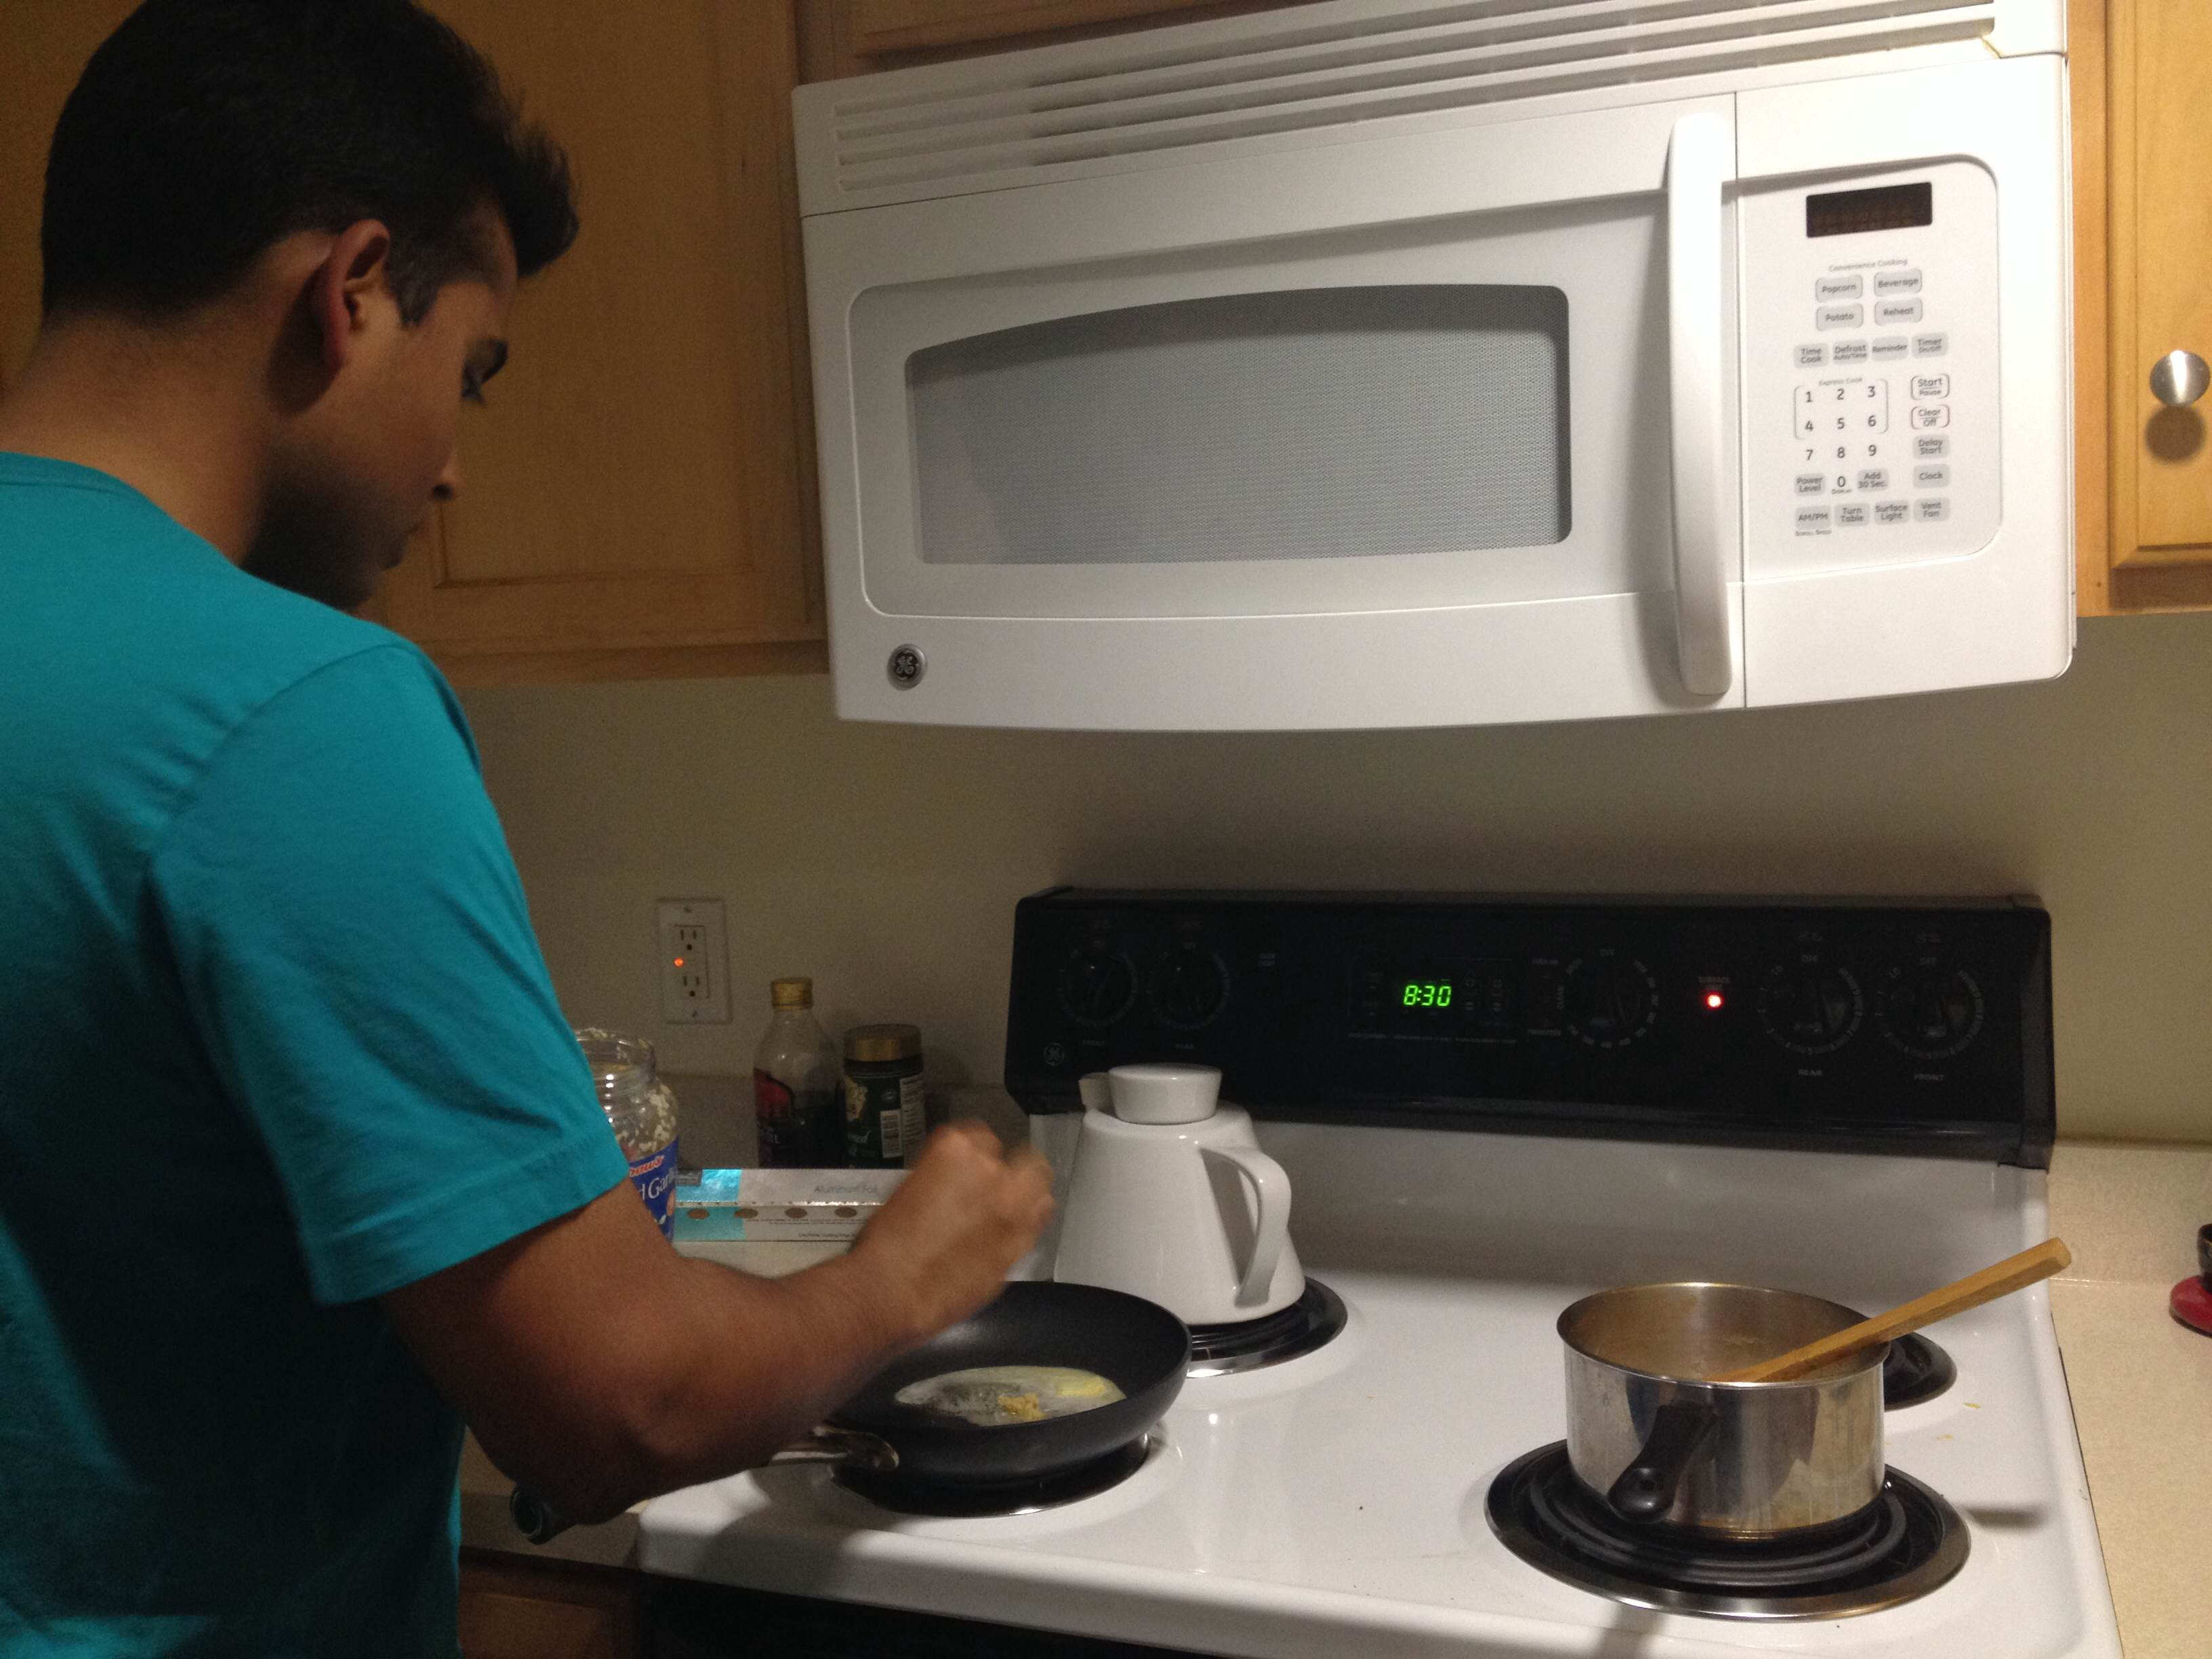
\includegraphics[trim = 0mm 0mm 0mm 0mm, clip,width=60mm]{IMG_4156.JPG}\\
  \caption{Observing Subject 1}
  \label{fig:subject1}
\end{figure}

\section{Initial Paper Prototypes}
The initial genesis of this project came when we noticed there was not a significant transformation of recipe presentation by means of technology. Initially, we developed several low fidelity paper prototypes in order to gain early insights into a design. Figure \ref{fig:paper1} shows an example of our paper prototypes overviewing a recipe interface, and Figure \ref{fig:paper2} illustrates a single step of the recipe interface. Initially, we envision to add features such as text-to-speech instruction, timer for managing multiple simultaneous tasks, reminders to check oven and stove temperatures, and many other features that can be assisted by advanced technologies. However, as we progressed our experiment, we realized there were more fundamental issues in traditional recipe presentation. The next section describes our experience observing novice chefs cooking, and presents fundamental challenges in traditional recipe presentation.

\begin{figure}[tbh]
  \centering
  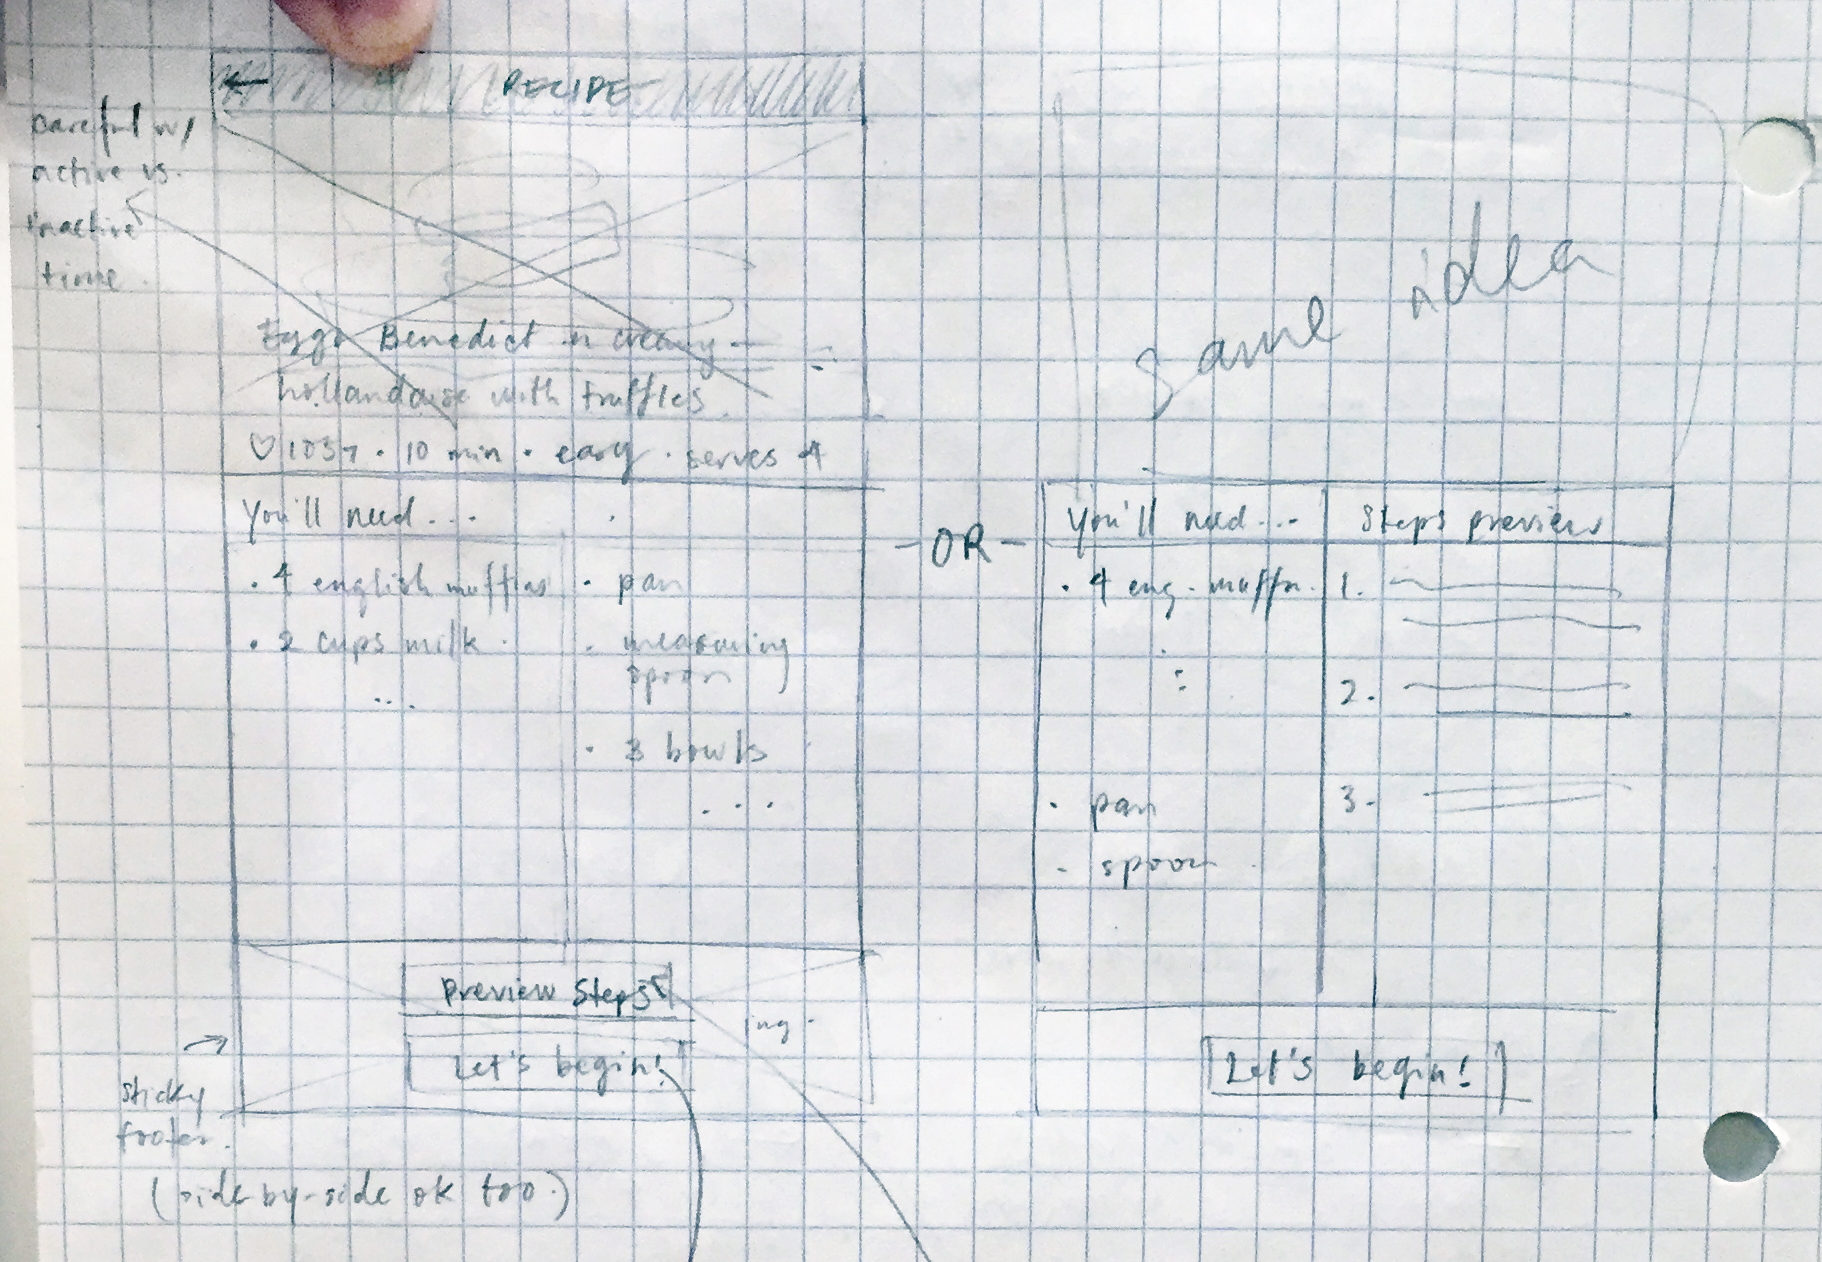
\includegraphics[trim = 0mm 0mm 40mm 0mm, clip,width=60mm]{recipe-overview.jpg}\\
  \caption{Recipe Overview Interface}
  \label{fig:paper1}
\end{figure}

\begin{figure}[tbh]
  \centering
  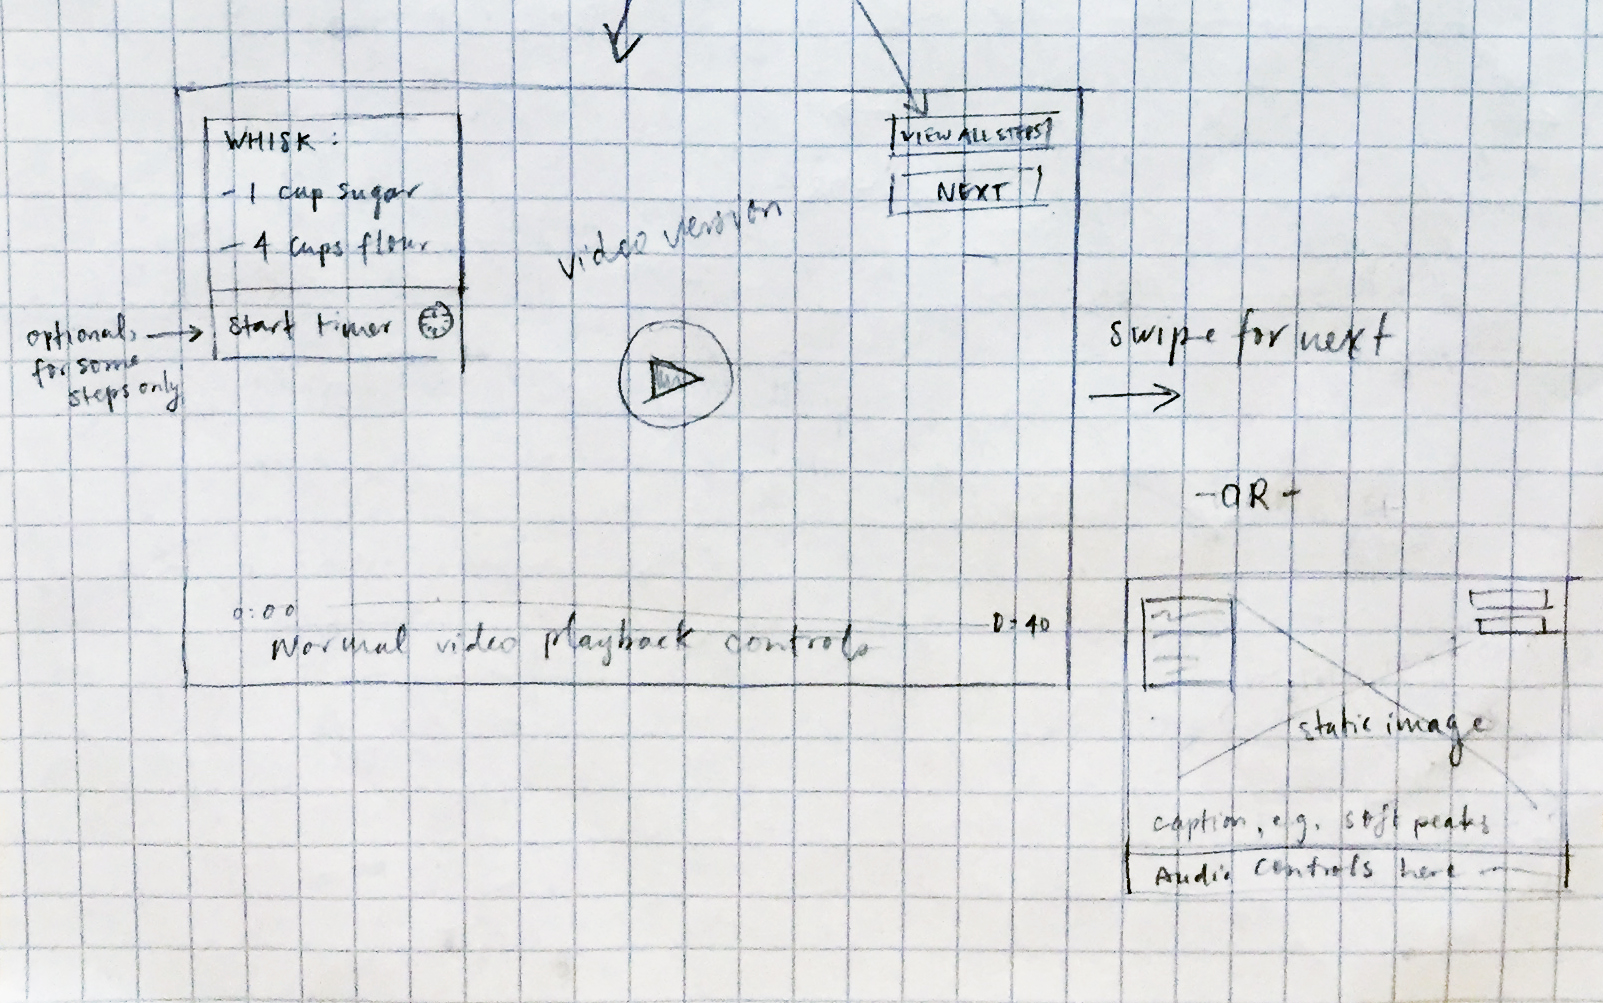
\includegraphics[width=60mm]{recipe-step.jpg}\\
  \caption{Recipe Step Interface}
  \label{fig:paper2}
\end{figure}


\section{User Study \#1}
For the first experiment, we observed three subjects. The experiment was conducted as follows: each subject was asked to cook a dish that he/she had never made before. We asked subjects to narratively describe the process that they are taking. The subjects' responses, behaviors, and surroundings were documented and occasionally recorded on pictures and videos.

\subsection{Subject 1}
Subject 1 had very little experience in cooking. His primary source of meal was delivery or prepackaged food. For the experiment, the subject was asked to cook Ravioli with Creamy Sun-dried Tomato and Basil Sauce \cite{cooking_classy}, which the subject had no prior experience in cooking. 

One of the first things we noticed upon observation of the subject was the organization of ingredients. Prior to cooking, the subject put out all ingredients that were listed in the recipe and measured their accurate portions. Even though all ingredients were measured accurately \textit{in the beginning}, he roughly guessed portion of ingredients using mugs and bowls \textit{while cooking}. After preparing all ingredients, he started boiling ravioli with sliced tomatoes. There were minor confusions on how much water to put in to cook ravioli and what shape tomatoes need to be cut but these issues were easily resolved based on the subject's prior experience and analyzing the final image of the dish. 

Every time the subject completed a task (e.g., slicing tomatoes), he looked at the recipe, found the position of the task he has just completed in the paragraph, and read the next step. Over the course of cooking, he looked at the recipe more than 20 times where each reading took a good amount of time trying to find the position of the step he has completed in the paragraph. The subject remarked, ``I have to constantly read over the paragraphs to see what step I am currently on.'' One interesting observation is when the subject did not look ahead. The subject mistakenly used all ingredients when some were needed again in later steps. The subject commented: ``My assumption is, unless it is specifically stated to save some for later, put all ingredients in. It would have been helpful if recipe is structured in a form that is easier to see what ingredients are coming ahead." While closely reading individual steps were well-comprehended, coordinating such task while multitasking did not work well at all. Evidence of this was given when the subject was missing steps.

After cooking, we found that all ingredients (including the ones that were no longer needed) were kept in open air as shown in Figure \ref{fig:open_ingredients}. The ingredients were kept open and outside for an additional hour even after the completion of cooking. 

\begin{figure}[tbh]
  \centering
  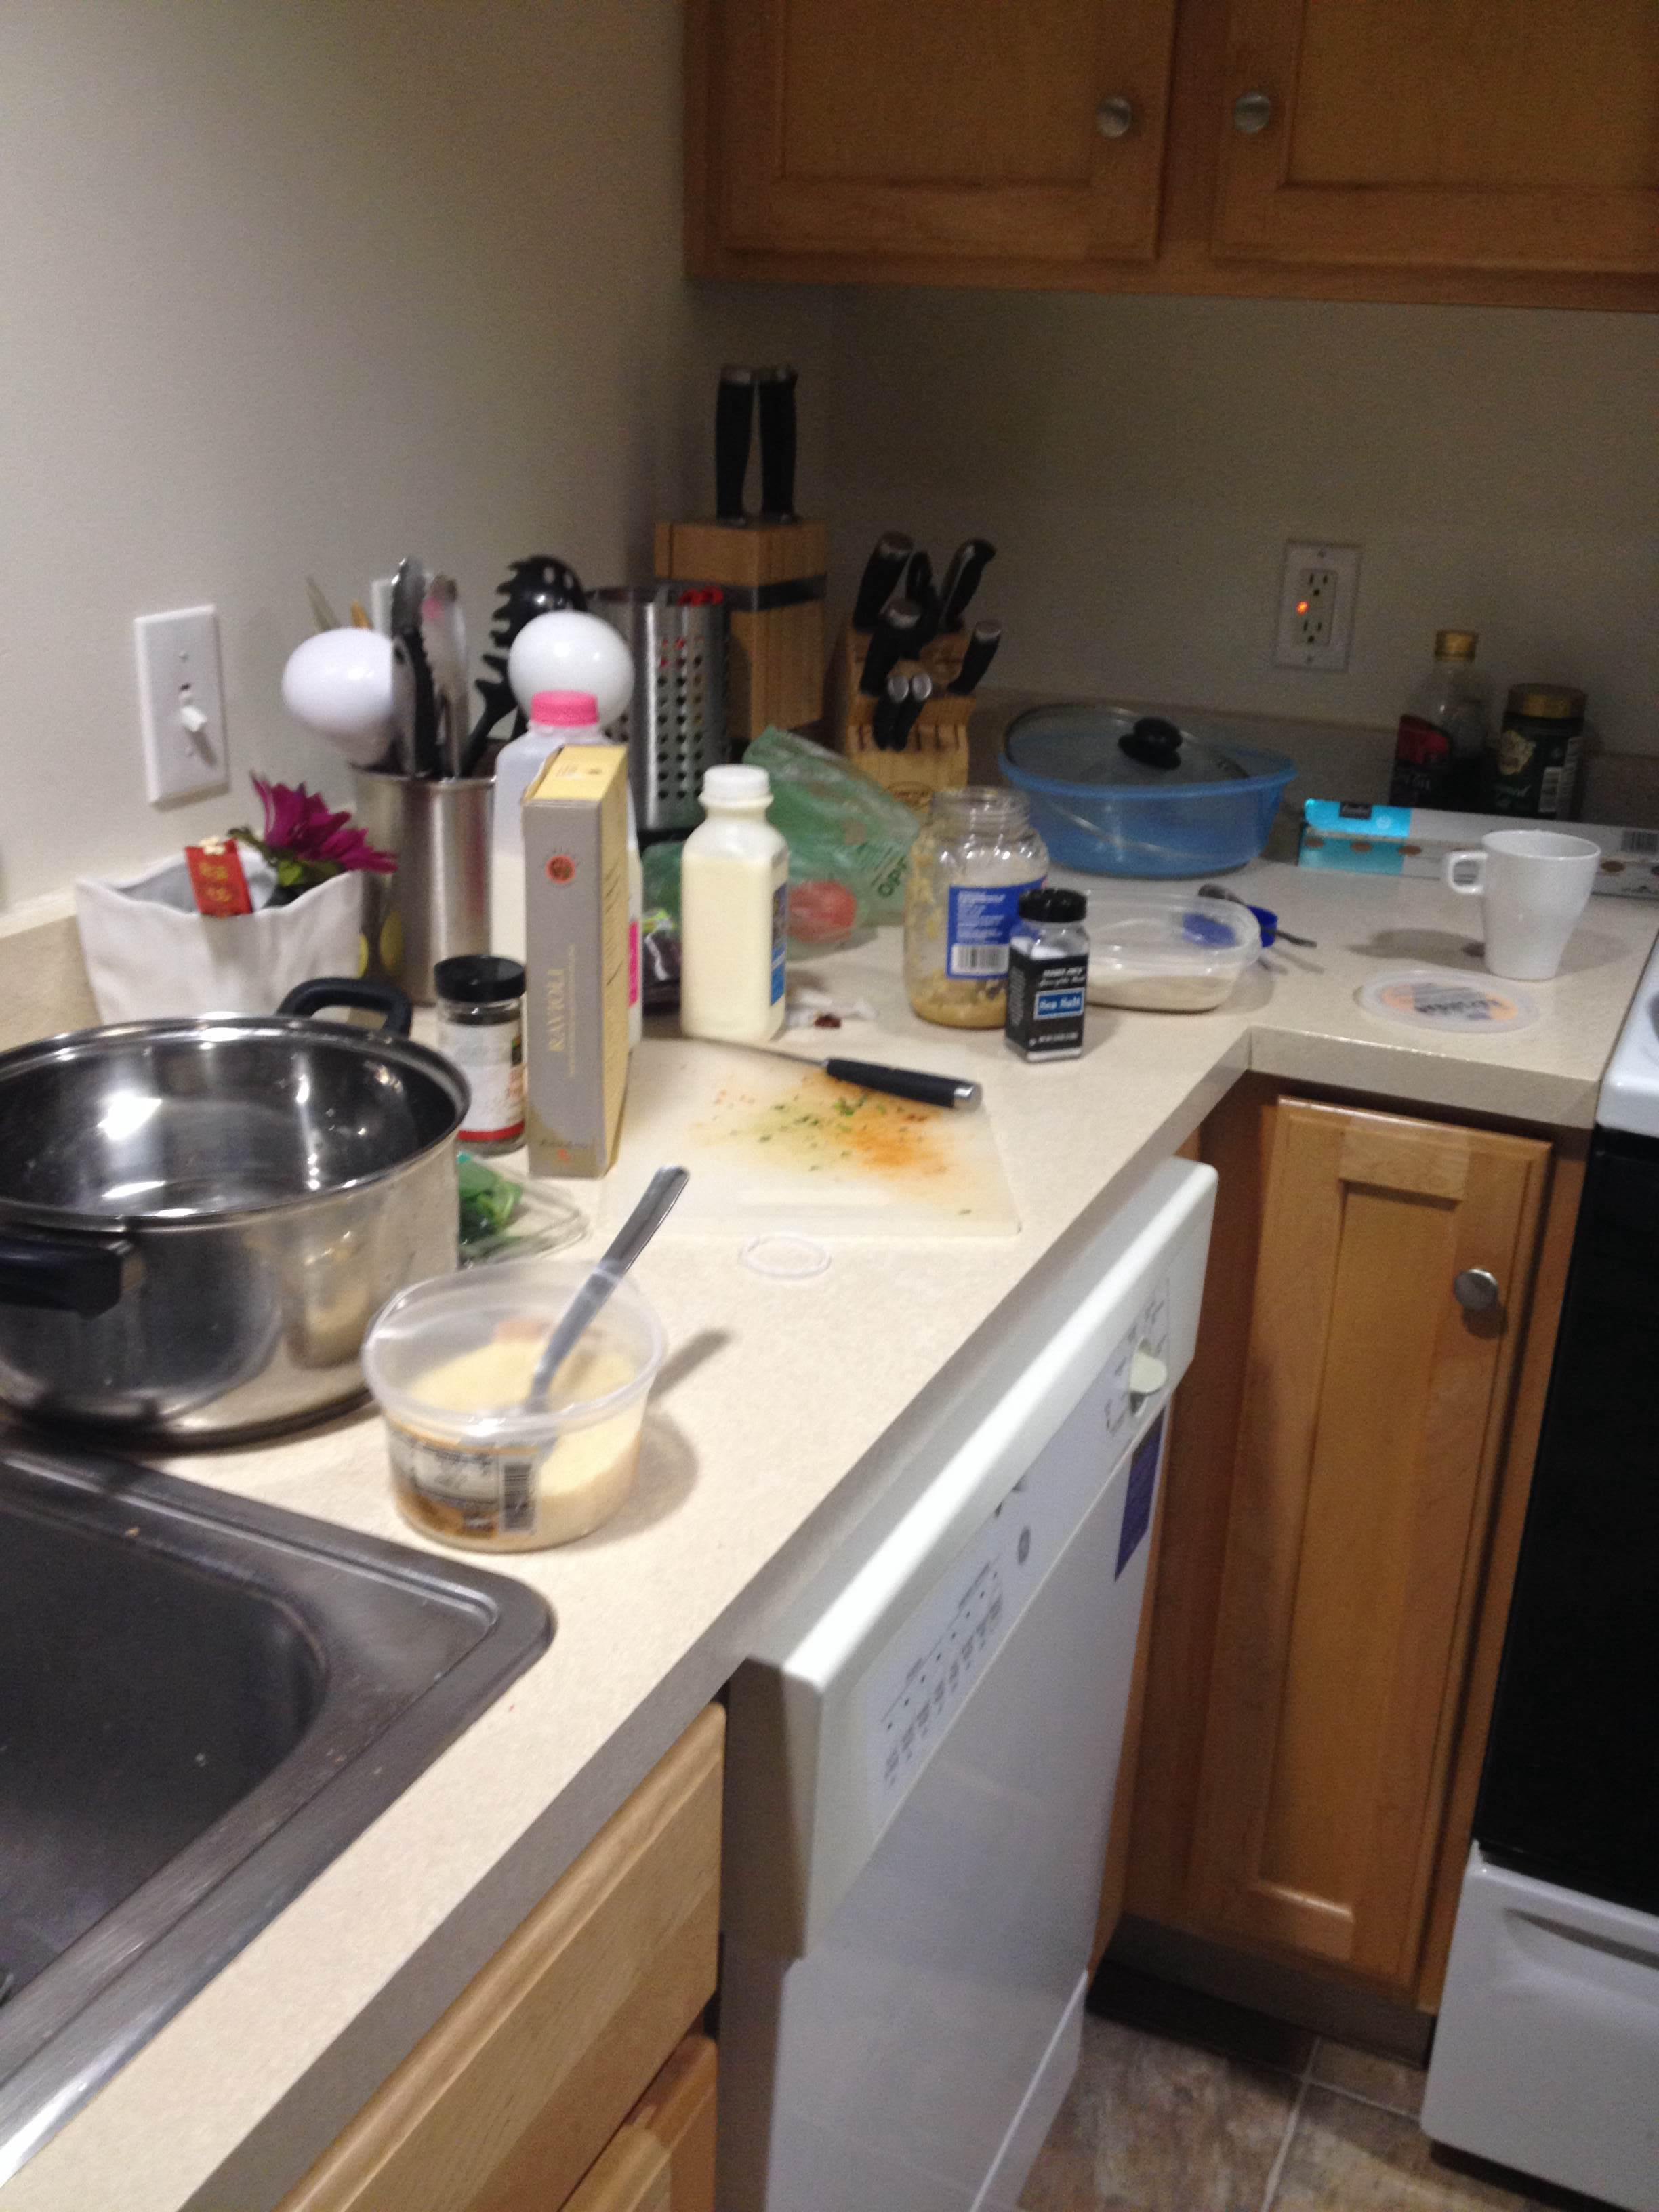
\includegraphics[trim = 0mm 250mm 0mm 100mm, clip,width=60mm]{IMG_4173.JPG}\\
  \caption{Ingredients were kept open and outside}
  \label{fig:open_ingredients}
\end{figure}

%Key observations are:
%Put all ingredients out and measured ingredients accurately in the beginning but roughly estimated using mugs and bowls while cooking 
%Unsure of cutting shapes 
%Used resulting images to decide on a shape
%Constantly looked at the recipe (> 20 times)
%Missed a step
%?I have to constantly read over the paragraphs to see what step I am currently on?
%Did not look ahead and mistakenly used up all ingredients when some were needed again in later steps
%?My assumption is, unless it?s specifically stated to save some for later, put all ingredients in?; ?It would have been helpful if recipe is structured in a form that is easier to see what ingredients are coming ahead? 
%Multitasking: checking pasta boiling while preparing sauce
%Brought heated frying pan to other side of kitchen to read recipe
%All ingredients (including the ones that were no longer needed) were kept open and outside



\subsection{Subject 2}
Subject 2 was a relatively experienced cook. The subject was asked to make Spaghetti Squash Gratin \cite{martha}. She had experience roasting spaghetti squash, but had no prior experience preparing this recipe.

She spent about one minute reading instructions and realized that Roasted Spaghetti Squash ingredient required significant preparation. After preheating oven and heating water, she read instructions again to scan for instructions that could be done while the oven preheats and the water boils. After preparing for all ingredients, she read the entire recipe again, from beginning, to re-evaluate her process. The subject continuously multitasked while cooking (e.g., prepped flour while waiting for liquid solution to reboil). Timer was used only for ingredients that may burn (e.g., warming milk). While cooking, she continuously read the recipe to to reassess her own mental process for cooking the recipe.

Similar to Subject 1, Subject 2 repeatedly read/scanned entire recipe, often standing idle, contemplating how to go about executing recipe. Time spend reading the recipe ranged from 30 to 90 seconds. Unlike Subject 1, Subject 2 took more control over reading the recipe instruction, and did not completely rely on the presented ordering of the recipe. Furthermore, Subject 2 reviewed past instructions to determine if she has made any mistakes. While observing the subject, we realized there was a significant gap between the number of steps carried out by the subject and the number of steps.

While whiskering flour into liquid solution, she encountered unexpected situation where flour started clumping. Later, she realized that the amount of sage she used was incorrect. Similar to Subject 1, Subject 2 read individual steps of recipe multiple times, however coordinating instructions while multitasking led to mistakes in keeping track of active ingredients. 

Subject 2 was relatively comfortable improvising instructions for current needs. For example, when pot called by recipe was too small, she improvised by mixing spaghetti squash and liquid/flour mixture in a larger container. 


%Key Observations:
%1) Most ingredients were "prepped," meaning a process exists from taking the raw ingredient to the prepped ingredient (e.g. "baked spaghetti squash" as an ingredient).
%2) Subject repeatedly read/scanned entire recipe, often standing idle, contemplating how to go about executing recipe. 
%3) Material (pot size) called for by recipe was incorrect (too small).
%4) Timer was only used for items that may burn (warming milk).
%5) When asked, subject stated she preferred recipes that structure preparation process.
%6) Recipe was read ~11 times, but time spent reading recipe ranged from 30 to 90 second periods. 
%7) A significant gap was observed between the number of steps carried out by the subject and the number of steps.


%Subject picked a small pot, filled with water, and began heating to boil. She spent about one minute reading instructions and realized that Roasted Spaghetti Squash ingredient actually required significant preparation. After preheating oven, subject read instructions again to scan for things that could be done while the oven preheats and the water boils. Whatever could be prepared was prepared ahead of time. When oven preheats, puts squash in.
%
%At this point, subject actually starts carrying out steps specified in instructions: Water boils, adds mixture and ``whisks." 
%
%Subject looks at past instructions to determine if she has made a mistake. When squash done, most other ignredients have been prepped. Subject reads the entire recipe again, from beginning, to re-evaluate her process. While waiting for liquid solution to reboil, subject preps flour. 
%
%Only time she uses a timer is for liquid solution, because it contained milk, which burns easily. Read recipe again to reassess her own mental process for cooking the recipe.
%
%``Whisked" flour into liquid solution (which was done boiling). Flour was clumping, which was unexpected (``this is not good"). Melted butter in pot, added flower/liquid mixture to pot. Noticed that amount of sage she used was incorrect, so had to remeasure sage. Subject had to add squash to pot, but pot called for by recipe was too small. 
%
%Subject improvised by mixing spaghetti squash and liquid/flour mixture in a larger container. Subject poured mixture into baking container, sprinkled remaining ingredients over mixture, and baked the final mixture. A timer was used for this last step.
%
%*****write in a paragraph form



\subsection{Subject 3}
Subject 3 also had some experience in cooking. The subject was asked to make Mushroom Ravioli with Goat Cheese from scratch \cite{goodfoodstories}. The subject did not have prior experience making the dish and unexperienced working with dough.

Subject began by skimming both recipes. He commented that he likes to ``parallelize" when cooking to minimize time spent, and to do that, he 
needs to read all steps a few times to process them and decide what to do first. Noting that the filling needed to cool before being wrapped,
and that the dough preparation really only had 20 minutes of downtime, he decided to first prepare the filling and then move on to the dough.

The subject referred back to the 
recipe at least twice in each step, often once every couple of ingredients (and some steps had many ingredients), to double check the quantity 
and amount of time necessary to process each. Each time he checked the recipe, he only glanced at it a second or two, skimming for key numbers.

Making and rolling dough was a challenge, because the subject had never before worked with pasta dough. Here, he still followed the 
recipe step by step, but referred to it more to understand how to work the dough rather than what to put in it. As a result, each recipe
check was longer and more involved; he read the sentences of the recipe and scrolled back and forth to check the pictures. 

Next came filling and wrapping the ravioli. He first unsuccessfully skimmed both recipes looking for specifics on the optimal ratio of filling to dough, as well as how large to cut the ravioli. He then Google searched quickly, before deciding that it was useless since nothing was to scale and decided to
just use ``gut" and his prior experience with Chinese dumplings. He did not need to consult wrapping instructions after that point.

The last step written on the recipe was to boil the ravioli. This he did without consulting the recipe. He did wonder aloud when the ravioli
would be done but decided that he'd just wait until a bit after they floated, like dumplings. As per his ``parallelization" tactic, he set the water
on a boil when he still had a few more ravioli to wrap so that he could get moving immediately when the ravioli were ready. He commented that it would 
be faster to have started boiling the ravioli in batches, while more of the ravioli were still unwrapped, but that it was unimportant because
boiling time was so short.




\subsection {Evaluation}
As a result of these observations we found that existing curation of a recipe was very difficult for the novice users to comprehend while cooking.  Subjects repeatedly read and scanned the entire recipe. Novice subjects had  a lot of difficulty remembering the current step within the paragraph and spent significant amount of time keeping track of current and upcoming steps. Additionally, there were poor connections between recipes that were parts of one dish. These observations were further corroborated in our interface evaluation. 

Based on these observations, we decided to focus on the curation of recipe instructions and ingredients. 


\section {System Design}

\begin{figure*}[tbh]
  \centering
  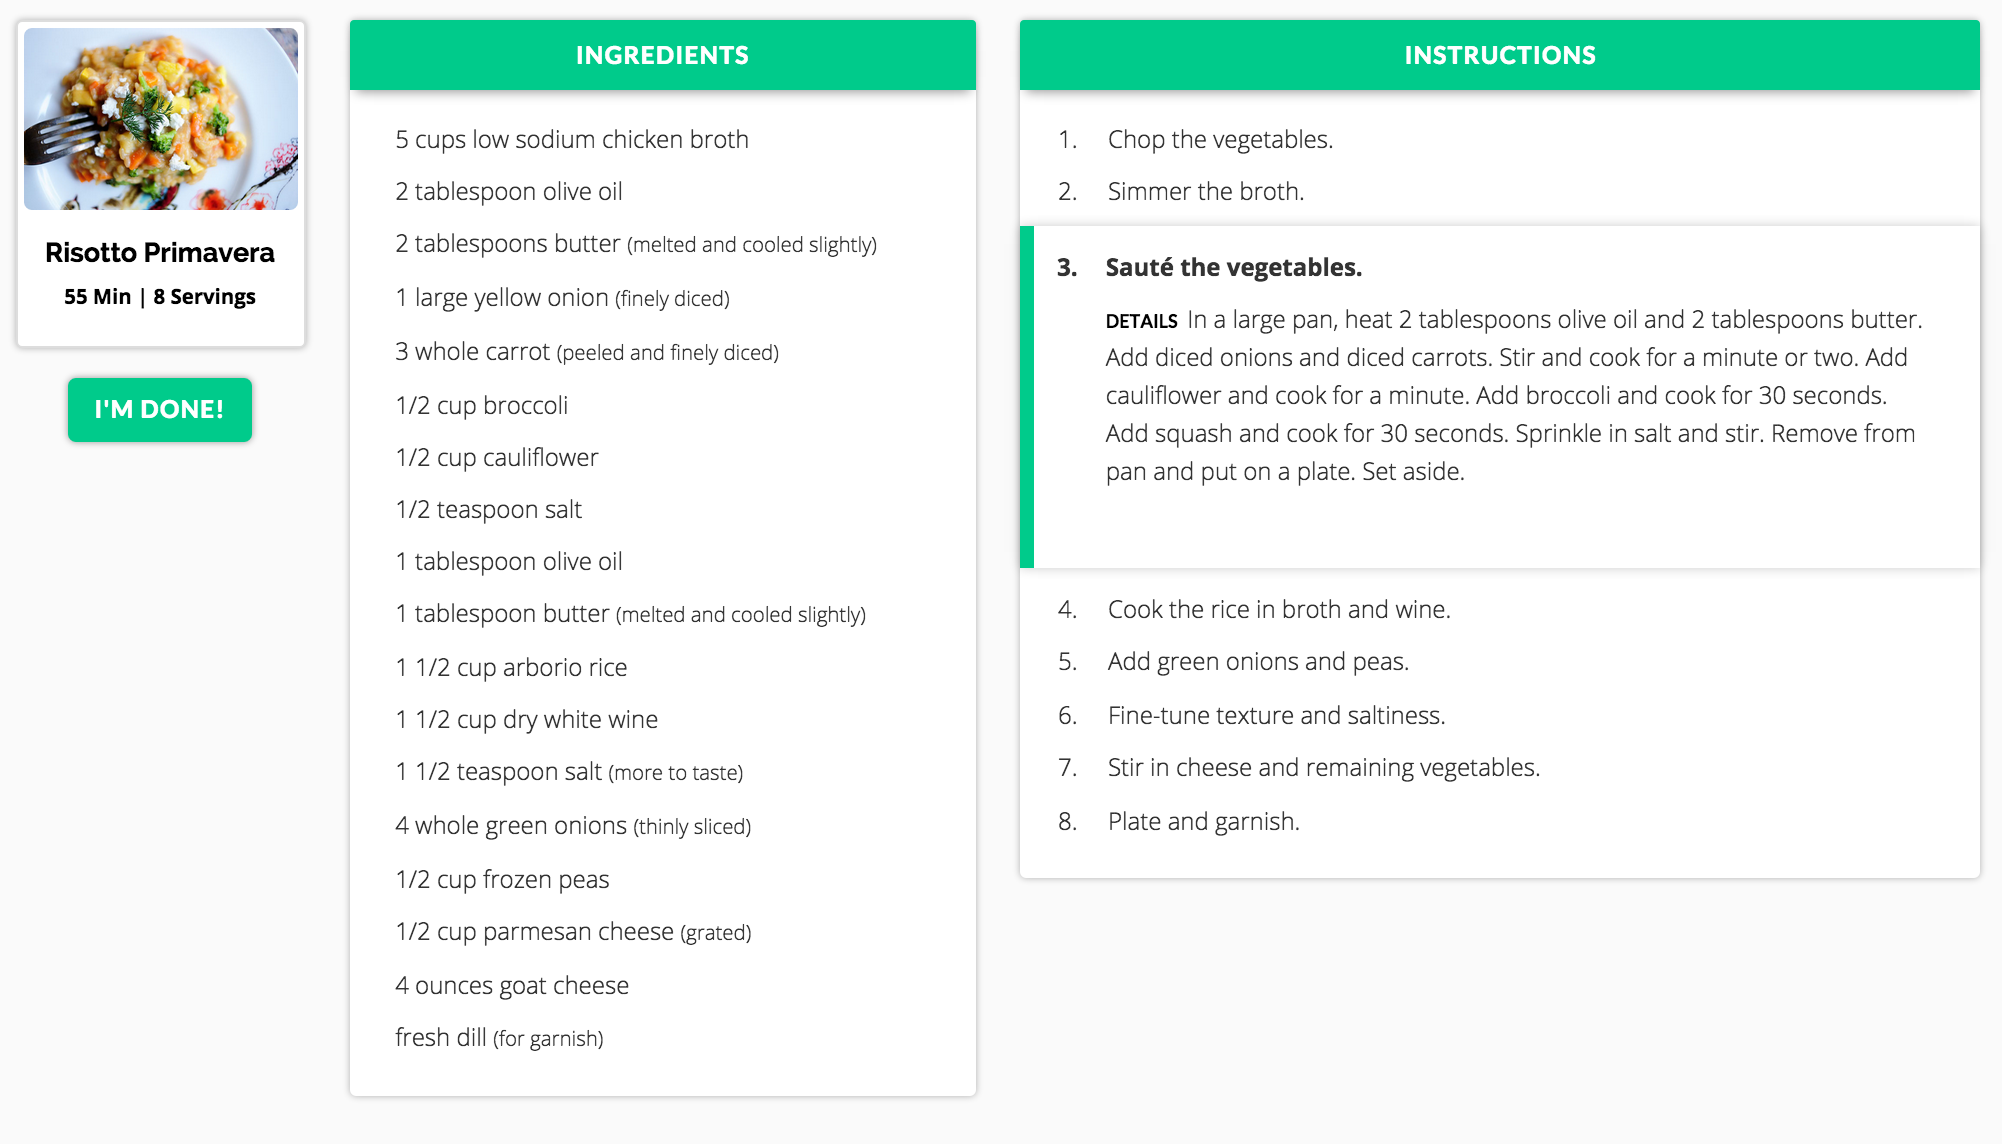
\includegraphics[trim = 0mm 0mm 0mm 0mm, clip,width=180mm]{ours.png}\\
  \caption{Example view of our proposed Responsive interface}
  \label{fig:ours}
\end{figure*}

After gaining this background knowledge, we developed a new interactive prototype that focused on curation of recipe instructions. From the user study, we found the difficulties of identifying current step in traditional recipe design. In our proposed interface, we included a feature that highlights the current step. We expect highlighting the current step will reduce the cognitive load of users, because they no longer need to scan the entire recipe to identify the step they have just completed. The position of the highlighted box remains consistent throughout the instructions. We further discuss the details of this feature in the later section. While highlighting the current step, our interface also presents the summary of previous and next steps. We have found that reviewing previous and future instructions is important for successful cooking but the traditional recipe design makes it difficult to quickly review the steps. For that, we design our interface to only include the summary. An example view of our proposed interface is shown in Figure \ref{fig:ours}.

In order to compare effectiveness of different recipe interfaces, we developed three interactive web-based interfaces: traditional recipe interface, step-by-step interface, and our proposed interface. Figure \ref{fig:control} shows the traditional recipe interface curated as a list. Step-by-step interface is commonly used for cellphone-based recipe interface. As shown in Figure \ref{fig:stepbystep}, it presents a single step at a time and allows user to click next or previous to navigate the instruction. 

\begin{figure}[tbh]
  \centering
  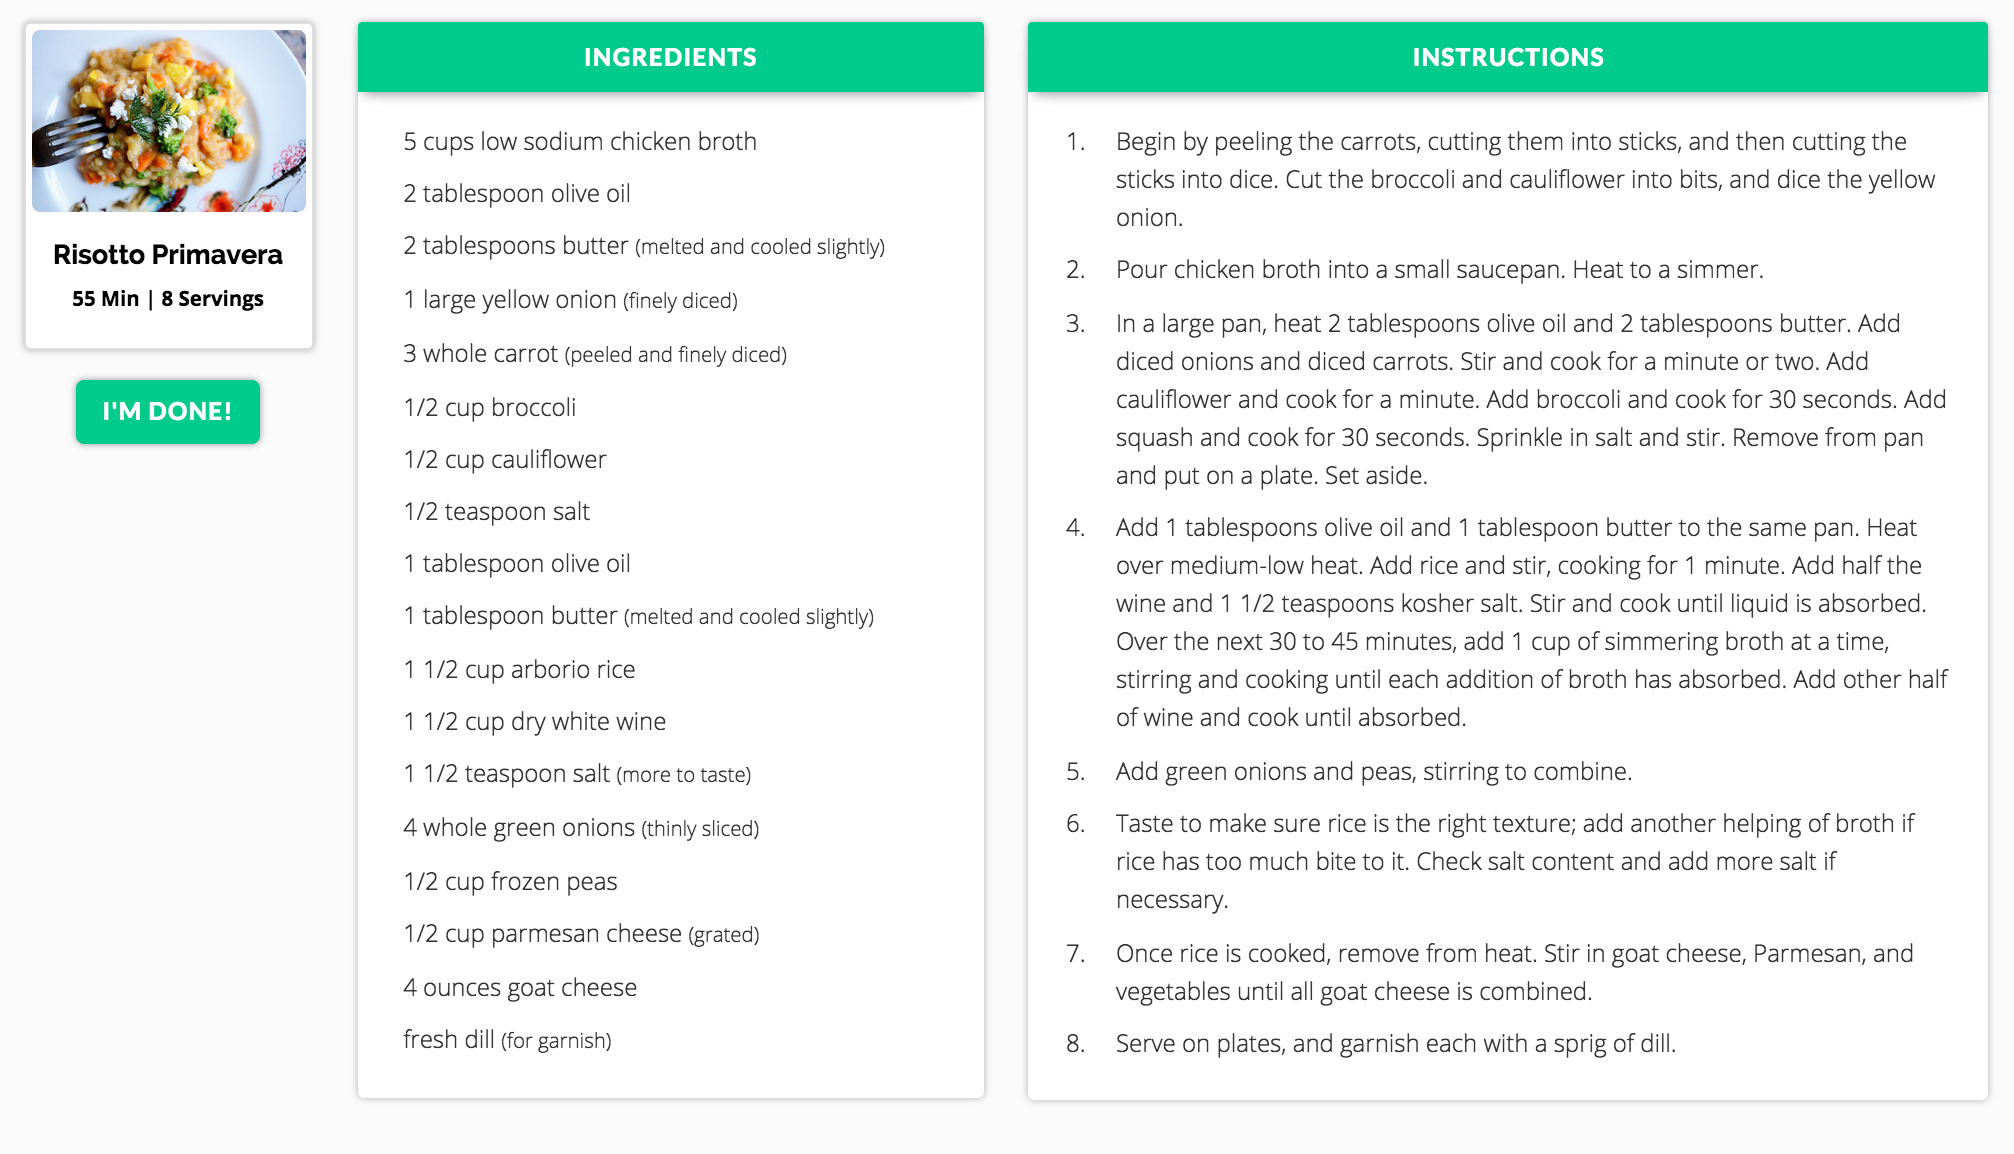
\includegraphics[trim = 0mm 0mm 0mm 0mm, clip,width=85mm]{control.png}\\
  \caption{Traditional interface of a recipe}
  \label{fig:control}
\end{figure}

\begin{figure}[tbh]
  \centering
  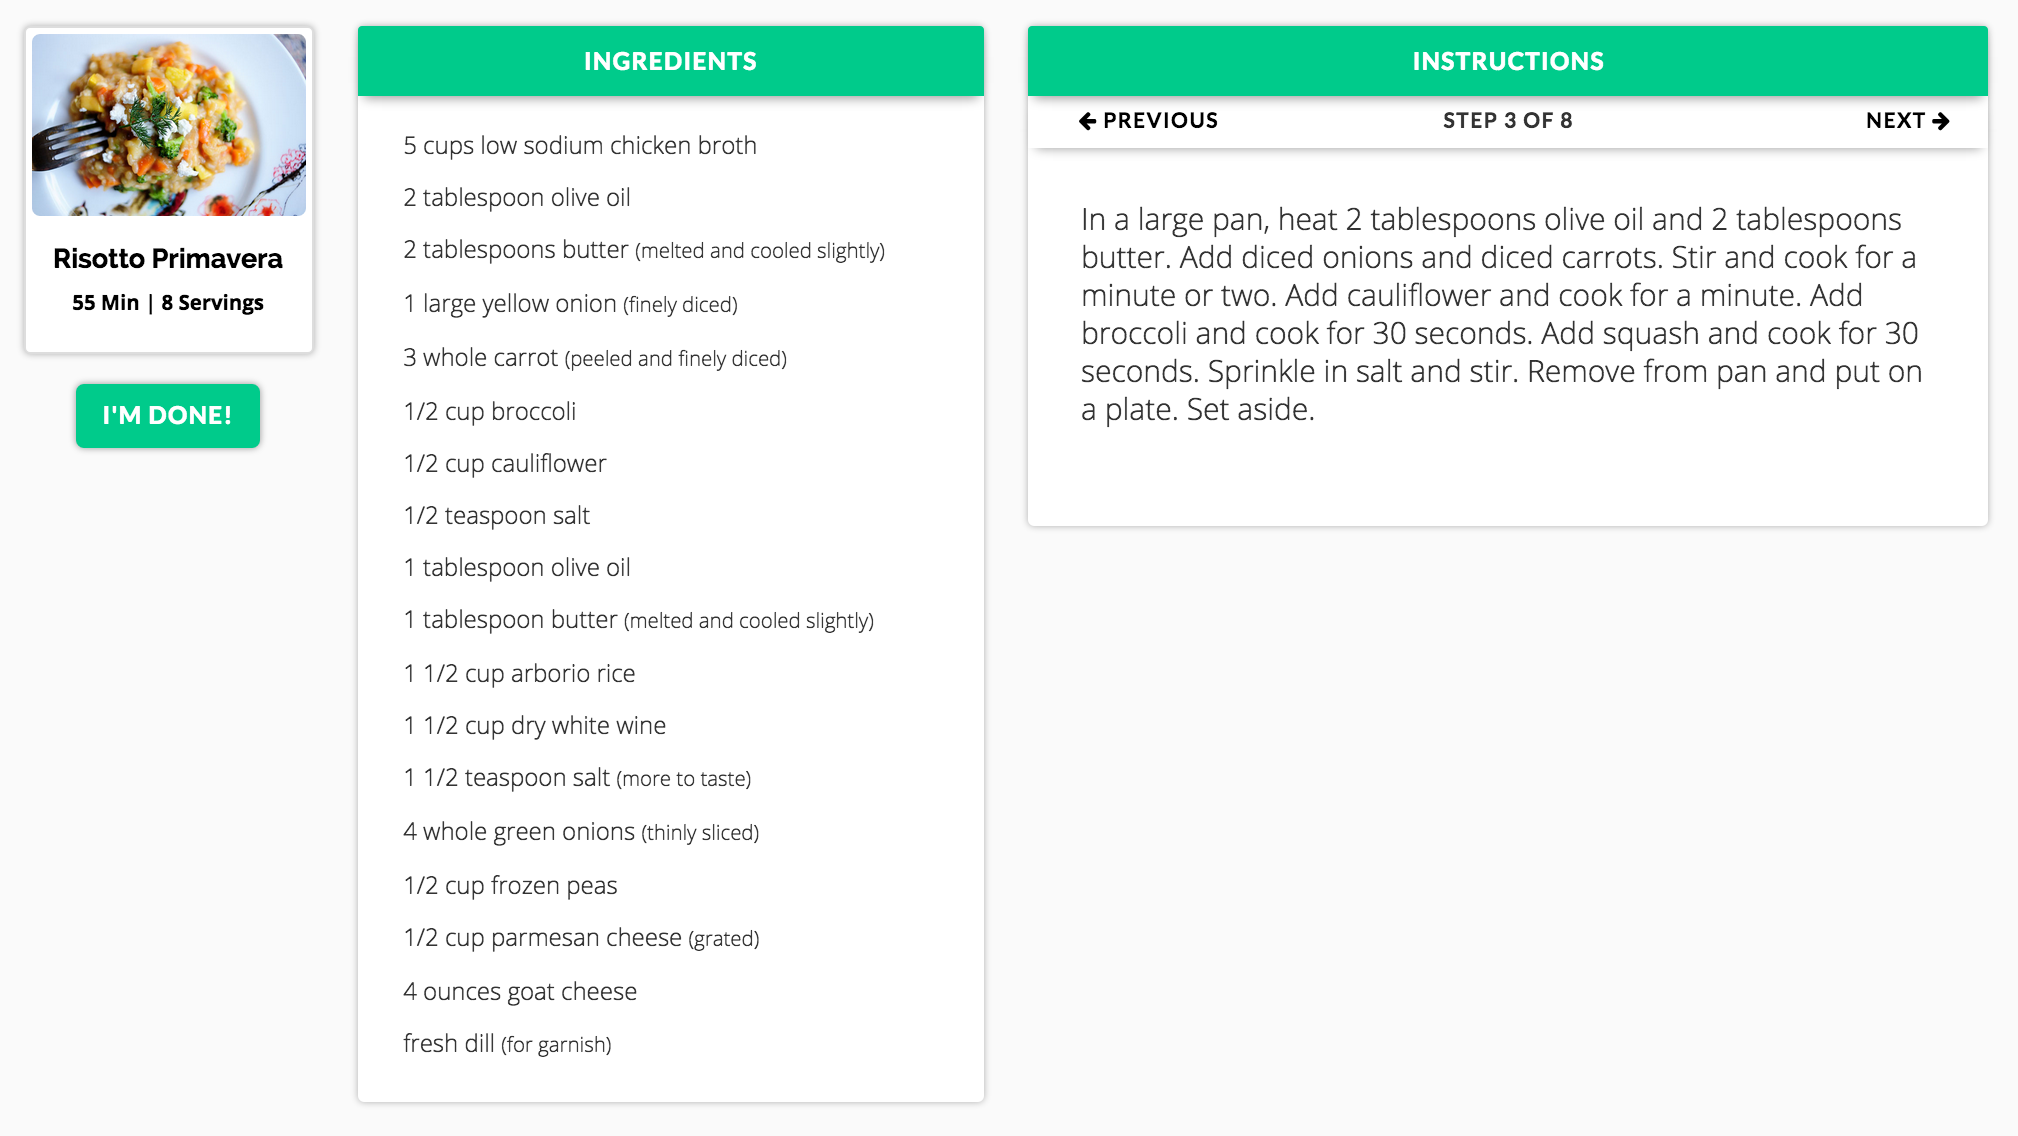
\includegraphics[trim = 0mm 0mm 0mm 0mm, clip,width=85mm]{stepbystep.png}\\
  \caption{Step-by-step interface that is commonly adopted for cellphone applications}
  \label{fig:stepbystep}
\end{figure}

\section{User Study \#2}
Three subjects are observed and interviewed for this study. Each subject was asked to test three interfaces (Control, Step-by-step, and our proposed Responsive interface). We curated three recipes (risotto primavera, mushroom lasagna, and baked eggs with spinach and mushrooms) that the subjects did not have prior experience making. Subject 1 tested traditional interface with risotto primavera, step-by-step interface with baked eggs, and our interface with mushroom lasagna. Subject 2 tested traditional interface with mushroom lasagna, step-by-step interface with risotto primavera, and our interface with baked eggs. Subject 3 tested traditional interface with baked eggs, step-by-step interface with mushroom lasagna, and our interface with risotto primavera. We measured time spent on completing individual steps as well as the entire instructions. Similar to User Study \#1, subjects narratively described the process that they were taking and the subjects' responses, behaviors, and surroundings were documented. Subjects completed NASA-TLX \cite{nasa_tlx} worksheet after each interface, and at the end of the experiment they selected their most preferred interface. 

\subsection{Subject 1}
Subject 1 tested Control, Step-by-step, and Responsive, respectively. The first recipe for Subject 1 was baked eggs with spinach and mushrooms using the traditional interface. Similar to User Study \#1, the subject accurately measured the ingredients in the beginning and estimated amount of ingredients used in each step while cooking. The subject stumbled on couple jargons such as `indentation' and `baking eggs.' The subject said his insecurity kicked in when he read the instruction, ``If baking eggs in this skillet, make 12 large indentations in mixture ... " because he did not know what baking eggs and making indentations mean. The subject said that the traditional interface presented too much information at the same time and remarked: ``This interface seemed like an essay.''

The second recipe was mushroom lasagna using Step-by-step interface. This interface also included ingredient highlighting feature that emphasized active ingredients in a step. We describe this feature in details in the following Section. When the subject first saw the interface, he expressed excitement because ``clear separation of steps made for easier digestion and awareness of what he needed to do without worrying too much of overall picture.'' He also stated: ``Even though the second interface was also in paragraph format just like the first one, it didn't have as daunting of a feel since it was just one." The subject also suggested that it would be nice to break down the paragraphs even smaller with more steps, although it would make it more challenging to go back and forth when doing simultaneous procedures. Throughout cooking, the subject had difficulty interacting with the interface because Step-by-step interface only showed a heap of information and was not easy to figure out intermediate steps. We found that ingredient highlighting made important information salient and removed extraneous information. The subject found ingredient highlighting very helpful. He remarked ``the highlighting of ingredients list as I went through the steps was wonderful because I could just focus on the few on table that I needed at the moment."

The third recipe was risotto using Responsive interface. This interface emphasized instructions for current step and highlighted ingredients for current step. The subject had much easier time multitasking using this interface. The subject said ``I liked that each step was clearly spaced out just like in second interface. But what made the third interface even better was I could see all the steps in one place rather than having to click back and forth multiple times to go from say step 2 to step 5 with interface 3. I could look at step 5 and then go back to step 2 with just one click." Because the subject was able to see summary view of the recipe, he said ``it sort of offered a little blurb/summary of what was being achieved in that step." The subject selected Responsive as his most preferred interface. 

\subsection{Subject 2}
Subject 2 tested Responsive, Control, and Step-by-step, respectively. The first recipe for Subject 2 was lasagna using Responsive interface. When first started the recipe, the subject scanned all the steps and went back to the first step. In the first step, the subject flipped to next step to have a sense of what could be done in parallel. The subject stated ``I was going up and down because I was trying to parallelize process." The subject found ingredient and instruction highlighting helpful but too coarse. He could not figure out which ingredients to prepare before others, or estimate how long each preparation process would take. Additionally, the subject suggested ``If the interface showed time or the number of pans you need per step, then that would be very helpful." 

The second recipe was risotto using the traditional interface. Looking at Control interface after Responsive interface, the subject remarked ``this interface is definitely much harder." The subject commented that the list of paragraphs was an information overload. The subject was worried that he might miss a step or an ingredient so he read the recipe multiple times before he started. Similar to our observation in User Study \#1, the subject said Control interface was ``difficult to follow along" and ``never knew where he was in the recipe." For Responsive interface, he only had to press up and down arrows when trying to read ahead, but with Control interface, every time he wanted to look next or previous steps, he had to scan the entire paragraph to see where he was, which was ``more irritating." While cooking, the subject noted images or videos in each step would be helpful. 

The third recipe was baked eggs with spinach and mushrooms using Step-by-step interface. The subject liked visually having `next' and `previous' cues. In the previous test, when the subject first opened Responsive interface he immediately went to clicking `Done' button to go to the next step. However, in Step-by-step interface, he did not make that mistake due to visual saliency of `next' and `previous' buttons. He commented ``arrow keys are normally for power users." Interestingly, we also noticed that the subject had a sense of completion when he clicked `next' button after completing each step. In terms of instruction and ingredient highlighting, similar patterns were observed as for Responsive. 

\subsection{Subject 3}
Subject 3 tested Step-by-step, Responsive, and Control, respectively. Subject 3 first made risotto using Step-by-step interface. The first instruction of the recipe was to chop vegetables so the subject first chopped vegetables and moved to the second step. The second step was to boil broth for cooking rice. The subject reported that she could have chopped the vegetables while boiling the broth, and said ``I guess I could have looked at step 2 to see if there was anything I could have started in the next step." This was arguably a flaw in the design of Step-by-step interface. The interface only showed current step, which limited cognitive load but it did so at the expense of knowledge. Hence, it led to longest total cooking time compared to Control and Responsive interfaces. The subject made heavy use of ingredient highlighting. While going back and forth in executing a step, she looked at screen for ingredient measurements, then went back to preparing the ingredients. She remarked: ``I liked the highlighted ingredients because ingredients were broken down into chunks instead of having it all sitting there in front of me. It was easier to read." Ingredient highlighting feature was reducing search time of ingredient measurements and allowed the subject to focus on preparing ingredients. 

The second dish was baked eggs with spinach and mushrooms using Responsive interface. The subject found summary view in Responsive interface informative. She commented ``it was a nice way of conceptualizing what I was about to read as a whole; so I didn't have to read all the details. Otherwise, I would have to skim through the steps to get the main idea of the step." Similar to Step-by-step, she found ingredient highlighting useful as she could focus on ingredients that were bolded, instead of looking at all the other ingredients. Similar to Subject 2, she wanted to have a feature that listed materials used for each step. The subject selected Responsive as her most preferred interface. 

The final recipe was lasagna using Control interface. After using Step-by-step and Responsive that had ingredient highlighting feature, the subject complained that the control interface did not have the feature. The subject commented that compared to Responsive and Step-by-step, Control interface is very plain as it was non-interactive. The subject selected Control as her least preferred interface. 

\subsection {Evaluation}
From User Study \#2, we found that most subjects preferred Responsive Interface over Step-by-step and Control. Compared to Step-by-step interface that only showed a single step at a time, we found that presenting the summary view of the recipe in Responsive interface provided users a sense of control. All subjects expressed that ingredient highlighting in Step-by-step and Responsive helpful in keeping track of ingredients per step while staying out of their way. From the observation, we identified that Responsive interface reduced load of extraneous information presented at any given step. This observation was further corroborated with our quantitative data shown in Table 1. For each recipe, the number of times a step has changed can be interpreted as the amount of cognitive load the recipe demands. Table 1 shows the number of times user has switched between steps. For each recipe, Responsive interface led to smaller number of step changes than Step-by-step interface.

%%%%%%%%%%%%%%%%%%%%%%%%%%%%%%%%%%%%%%%%%%
\begin{table}
  \centering
  \caption{Number of times user has switched between steps}
\begin{tabular}{|l|c|c|c|c|}
  \hline
                        & Risotto    & Egg  	    & Lasagna \\ \hline\hline
  Control        &   -  &    -   &   -   \\ \hline
  Responsive                   &   6  &    10   &  34   \\ \hline
  Step-by-step           &   14  &    25   &   37   \\
  \hline
\end{tabular}
\end{table}
%%%%%%%%%%%%%%%%%%%%%%%%%%%%%%%%%%%%%%%%%%%%%%%%


User feedback indicated that Step-by-step interface chunked information and missed important future steps that slowed subject down. On average, subjects took 94.5 minutes to cook a recipe using Step-by-step interface compared to 89.8 minutes using Control interface. For a given recipe, we  expected Responsive interface to take least total cooking time compared to Control and Step-by-Step, but this was not evident from data as Responsive took 92.7 minutes on average. 

Initially, we included NASA TLX survey to get user feedback on different interfaces. However, we realized that the survey ended up reflecting reactions to recipe, not interface. We observed that subjects had most difficult time making lasagna. As expected, lasagna had the highest rating for mental demand (risotto: 2.67; eggs: 3; lasagna: 3.67) and frustration (risotto: 2; eggs: 3; lasagna: 3.67) in NASA TLX survey. Referring back to Table 1, the number of times a step has changed indicated the amount of cognitive load the recipe demands. As lasagna was identified as the most difficult dish, it had the highest number of clicks, eggs had the second highest, and then risotto for both Responsive and Step-by-step interfaces. 

\section {Final Design Iteration}
For the final design, we improved Responsive interface based on our observations and users' feedbacks in User Study \#2. 

**********Continue writing + Add a screenshot

- Most subjects requested presentation of cookwares along with instructions and ingredients. In this iteration, we incorporated the feature of cookware curation. 

- All subjects looked at the photo of the finalized dish to decided on intermediate steps that were not elaborated in the recipe. Most subjects commented that having a picture in each step would greatly help them understand latent instructions. With their request, we added images in each step. 

- In the final design, we clearly added `next' and `previous' button. In previous Responsive interface, those buttons were not visually presented bur rather implied. 

\section {Design Observations}

In this section, we describe added features of our final design, and some factors that led to its relative success. 

\subsection{Instruction Highlighting}

\subsection{Instruction Summary View}

\subsection{Ingredient Highlighting}

\subsection{Cookware Listing}

\subsection{Native Scrolling}

\section{Conclusions and Future Work}



%\section{Acknowledgments}
%
%We thank CHI, PDC and CSCW volunteers, and all publications support
%and staff, who wrote and provided helpful comments on previous
%versions of this document.  Some of the references cited in this paper
%are included for illustrative purposes only.  \textbf{Don't forget
%to acknowledge funding sources as well}, so you don't wind up
%having to correct it later.

% Balancing columns in a ref list is a bit of a pain because you
% either use a hack like flushend or balance, or manually insert
% a column break.  http://www.tex.ac.uk/cgi-bin/texfaq2html?label=balance
% multicols doesn't work because we're already in two-column mode,
% and flushend isn't awesome, so I choose balance.  See this
% for more info: http://cs.brown.edu/system/software/latex/doc/balance.pdf
%
% Note that in a perfect world balance wants to be in the first
% column of the last page.
%
% If balance doesn't work for you, you can remove that and
% hard-code a column break into the bbl file right before you
% submit:
%
% http://stackoverflow.com/questions/2149854/how-to-manually-equalize-columns-
% in-an-ieee-paper-if-using-bibtex
%
% Or, just remove \balance and give up on balancing the last page.
%
\balance

% REFERENCES FORMAT
% References must be the same font size as other body text.

\bibliographystyle{acm-sigchi}
\bibliography{sample1}
\end{document}
